\chapter{State of the Art}

\section{Introduction}

The purpose of this section is to give a high-level overview of common internet censorship mechanisms, the past and present landscapes of internet censorship in Ireland and Iraq, and a brief description of some circumvention tools. This review was conducted using publicly available information and data published on the internet.

\section{Censorship Mechanisms}

The following section is based primarily on information from the source \textit{RFC 9505
A Survey of Worldwide Censorship Techniques} \cite{rfc9505}. Any other information sourced from elsewhere is identified as such.

\subsection{IP Blocking}

\subsubsection{Shallow Packet Inspection}

Shallow packet inspection refers to the action of looking at the transport layer segment (packet) headers to implement censorship based on the transparent source and destination IP addresses and port numbers. The information visible in the headers allows a censor to block content via IP blocklisting.

This method is easy to implement in some routers, but difficult to implement in backbone or ISP routers at scale. It is usually implemented alongside Deep Packet Inspection using middleboxes.

Internet Protocol (IP) blocking is one of the most straightforward censorship techniques, but it is also very crude. To implement an IP blocklist, the censor will create a route in a router's flow table that instructs the router to drop any packets matching a set IP address. In IPv4, this is done as a /32 route, and in IPv6 as a /128. However, due to the limited amount of space in router flow tables, this means that only a limited number of IPs can be blocked at a time, making it difficult to scale.

IP blocking can also cause content over-blocking. Because many websites share the same IP address, blocking one IP address can lead to multiple websites getting blocked within a network. Censors also sometimes block a range of IP addresses, which can lead to more over-blocking.

IP blocking is often ineffective against Content Distribution Networks (CDNs) and services that are hosted using multiple load-balanced IP addresses. This is because when the server hosting the content being sent changes its IP addresses, the block list may not include this new IP address, and the packets are not dropped. VPNs are an excellent tool to circumvent IP blocking as it routes the packets through different servers, changing the source and destination IP addresses along the way. This makes it nearly impossible to stop IP blocked content from getting through, as the source and destination IP addresses can be different for every packet coming from the original blocked source.

IP blocking can either be implemented at a centralized level or at an ISP level. In Ireland, IP blocking is done at an ISP level to block certain illegal websites in accordance with court orders (see section 2.2 for more information). In Iraq, IP blocking is implemented at the ISP level under the directive of the Ministry of Communications \cite{freedomhouseIraqFreedom} (see section 2.3 for more details).

\subsection{DNS Interference}

DNS interference refers to the altering of responses from the DNS to block or filter access to certain content. This is usually done by either blocking the response, replying with an error message, or responding with an incorrect address. \textit{DNS Mangling} is a network-level technique of on-path interception where an incorrect IP address is returned in response to a DNS query to a censored destination. 

\textit{DNS Cache Poisoning} is an off-path technique in which a censor intercepts and replaces the legitimate response from an authoritative DNS name server with a spoofed IP address. Instead of allowing the real IP address of a site to reach the user, the censor replies faster than the real server, and that spoofed IP gets cached (perhaps by numerous recursive resolvers). Subsequent requests will then be redirected to an incorrect IP, normally leading to a warning page or a meaningless domain. In other cases, such as in Iran, the censor can merely block the response of the upstream resolver, so the accurate IP address is never transmitted.

\textit{DNS Lying} is the most authoritative approach, where a censor mandates that the DNS responses provided are to be different from what would actually be returned by the DNS server \cite{rfc9505}.

The above DNS interference methods require the censor to traverse a controlled DNS hierarchy for this mechanism to be effective. This mechanism can be circumvented by using a different publicly known DNS resolver that is not controlled by the censor. This mechanism can also lead to unintentional blocking in area's not controlled by the censor. For example, sometimes a user outside of the censor's region will be directed through DNS servers controlled by the censor, causing the request to fail. Considering all of this, DNS interference is not a very effective censorship mechanism.

\subsection{Deep Packet Inspection (DPI)}

Deep Packet Inspection consists of any kind of packet analysis beyond IP address and port number. DPI reassembles network flows to examine the application data section, and is often implemented using Middleboxes. DPI is often used for keyword identification, but this method can also determine packet size and flow timings to detect other forms of content, such as the difference between text or video packets. Although DPI has difficulty with encrypted data and is the most expensive form of censorship to implement, it is still the most powerful identification method and is widely used in practice \cite{rfc9505}.

\subsection{Transport Layer Security (TLS)}

Transport Layer Security (TLS) is a protocol that secures most web traffic in our modern-day internet. As more internet traffic has become encrypted, the way censorship is implemented had to adapt. When users use circumvention tools such as VPN's or proxy solutions, more common censorship techniques (such as IP blocking or DNS interference) are often unable to sufficiently block undesired content. As a result, TLS-based censorship became more common as this mechanism is able to deny access to specific sites or services without decrypting the actual TLS content. 

\subsubsection{Server Name Indication (SNI) Filtering}

SNI Filtering is a widely used form of TLS-based censorship. The SNI is a TLS extension in the client's handshake (ClientHello) that indicates the hostname of the server the client wants to reach. In instances of anything up to TLS version 1.3 (assuming no additional encryption extensions are used), the ClientHello is sent in unencrypted plaintext. This allows a censor to read the requested hostname and block the connection if it is on a blocklist \cite{SNIUnencryptedCloudFlare}. This technique is implemented by many countries, and since 2018, the governments of China, Egypt, Iran, Qatar, South Korea, Turkey, Turkmenistan, and the United Arab Emirates have implemented widespread SNI filtering or blocking \cite{rfc9505SNIBlocking}. The Great Firewall of China has \textit{"Long been censoring HTTPS in this manner"} by blocking connections that match forbidden hostnames in the SNI field \cite{GreatFirewallSNI}. 

The obvious way to circumvent SNI filtering is to encrypt the SNI. In TLS 1.3, this is introduced as encrypted ClientHello (ECH). Before ECH, there was an extension that allowed for the SNI to be encrypted, aptly named Encrypted Server Name Indication (ESNI). But using ECH or ESNI has led to overclocking as censors simply block all traffic using them. An example of this can be found again in China, where all ESNI or ECH traffic is blocked.

\subsubsection{TLS Fingerprinting}

TLS Fingerprinting is used to identify and block tools or protocols that a censor might want to block. The way a TLS ClientHello is structured is like a digital fingerprint that is unique to an application or library. Censors will collect known fingerprints and deploy Deep Packet Inspection rules to block or flag those TLS connections \cite{TLSFingerprinting}. For example, a regime might recognize the unique CLientHello packet of Tor's TLS and configure the network to drop any matching packets. This technique, which is known to be used in China and Iran, prompted Tor to develop more mimicry in its TLS handshake. Many other circumvention tools followed this example, and have since tried to camouflage their TLS handshakes to look more like those of a common browser \cite{TLSFingerprinting}.

\subsection{Network Blackouts}

A very straightforward, holistic, and blunt form of censorship is network blackouts. This method involves a large governing body of an area or region completely shutting off Internet access for all content. This method is becoming more and more common across areas in the Middle East and Asia. According to a report from \textit{Access Now}, there were a total of 296 different internet shutdowns across 54 countries. This is a 35\% increase from the previous high in 2022 \cite{inetenetBlackouts}. This form of censorship is very extreme and is often implemented in times of conflict, protest and instability, exams, and elections. 

\section{Ireland}

\subsection{Censorship in the Past}

According to a report from the United States Department of State in 2011, it was found that there were no government restrictions on access to the internet or that the government actively monitored email or internet chatrooms \cite{stateTechnicalDifficulties}.

The Irish government engages in censoring or blocking the distribution of pirated copryrighted material. In 2009, the Irish Telecom Company, EIRCOM, blocked its customers from accessing the website \textit{The Pirate Bay}. The Pirate Bay is a Swedish website which provides links to copyrighted material. The website was hit with a lawsuit from major record labels and many ISPs around the world agreed to block access to the website as part of the settlement. However, not all Irish ISPs complied. The cable TV operator UPC announced that it would not comply \cite{irishtimesEircomBlock}. 

In alignment with international agreements, the Irish Government blocks access to websites that contain illegal content, such as Child Sexual Abuse Material (CSAM). The government has setup a hotline that allows citizens to anonymously report websites that they suspect contain illegal content, called hotline.ie \cite{hotlineAboutx2013}.

In contrast to other EU countries, Ireland does not have a broad government-mandated filtering system. They instead have the power through the Irish courts to mandate Irish ISPs to block certain websites. In addition, Irish ISPs may voluntarily enforce content filtering and website blocking in alignment with Irish content law.

Up until 2014, Ireland and other EU countries followed data retention laws, which required ISPs to store metadata for law enforcement purposes. In 2014, the European Court of Justice struck down the directive, which led to a change in this law in Ireland \cite{DataRetentionInvalid2014}. After this change, Ireland enacted the \textit{Communications (Retention of Data)(Amendment) Act 2022} \cite{irishlegalDataRetention}. This legislation allows for the general and indiscriminate retention of communications traffic and location data on the grounds of national security, where approved by a judge.

\subsection{Current Censorship}

As a whole, Ireland's censorship efforts are limited and specific. The government and ISPs target mainly illegal and pirated content. Some specific websites that have been blocked include 1337x, Eztv, BMovies, GoMovies, Putlocker, Rarbg, WatchFree, and Yts \cite{siliconrepublicMovieIndustry}. However, piracy websites are still widely accessible in Ireland.

It seems that Ireland has also rolled back blocks on some websites, such as Russian News outlets. Previously, the domain russia.tv, was blocked in Ireland. But as of 2025, it is able to be partially accessed. Based on data from the OONI project, there is evidence of TCP/IP blocking of this domain in Ireland. Based on the findings from OONI, this domain is able to be accessed when EIRCOM's root DNS server (AS5466, IP: 86.47.80.38) is used, but is blocked when accessed through Cloudflare's DNS server (AS14593, IP: 172.69.193.80).

\centerline{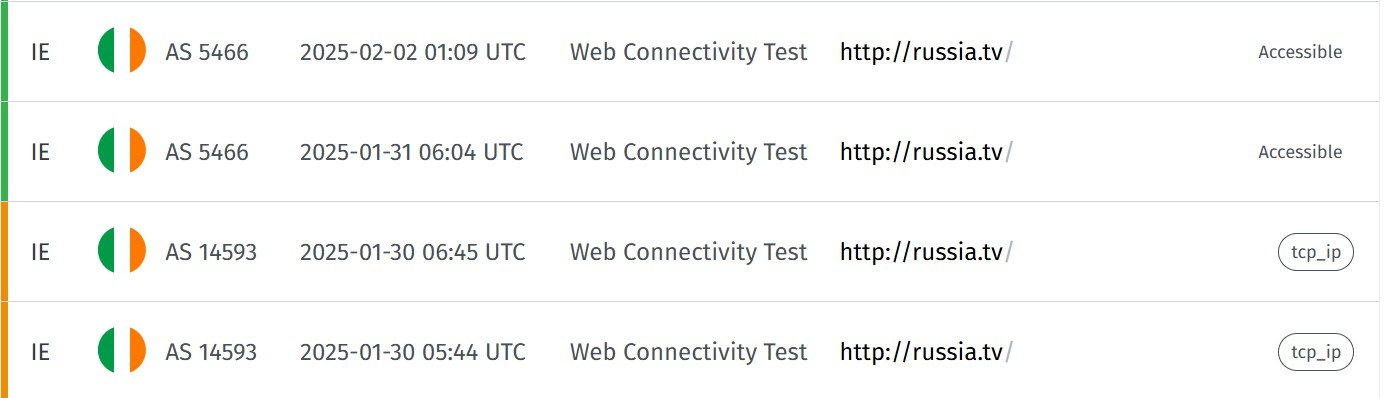
\includegraphics[width=480pt]{Griff/TCD SCSS CAPSTONE/Literature Review/RussiaTV search OONI.jpg}}

\centerline{\textit{Figure 1.1, Russia.tv domain search on OONI}}

\section{Iraq}

\subsection{Censorship in the Past}

Iraqi internet censorship has been radically reshaped over the years. Under Saddam Hussein's regime, only a very few Iraqis had access to the internet, leading to the state controlling all parts of the internet within the country. Post-2003, with more people accessing the internet and the country struggling with internal conflict and the threat of radicalization, censorship was decentralized and usually carried out with little transparency and regionally differentiated. While the constitution and laws of Iraq recognize free expression, actual enforcement is usually slow whenever security is at stake. As the internet began to take a greater role, both as a platform for political discourse and a vehicle for extremist messaging, the censorship and intrusions of the government increased correspondingly. Generally speaking, the policy of controlling the internet in Iraq has mirrored the broader political and security situation, tightening whenever Iraq is unstable \cite{freedomhouseIraqFreedom}.

Historically, most of Iraq's censorship was implemented via DNS interference and IP Blocking. In 2014, a Citizen Lab test found around 20 URLs that were blocked, likely by DNS interference, and displayed a government block page. In these tests, when a user tried to visit a banned site, they either got an incorrect DNS resolution or their HTTP request was outright blocked \cite{citizenlabIraqPastCensorship}. In 2014 TLS usage was much lower so DNS and IP blocking was more effective. 

\subsection{Current Censorship}

Iraq's internet growth has progressed from state-controlled limitations during Saddam Hussein's era, where limited citizens used the internet. After 2003, many private ISPs were formed, but primary fiber routes and gateways that link Iraq to international submarine cable networks via adjacent countries are still controlled by the Ministry of Communications \cite{IraqCMC}. Baghdad, the country's capital and commercial center, is a hub of national connectivity, and other large cities (like Basra and Mosul) typically have local backbones that connect into the national fiber network. The Kurdistan Region of Iraq (KRI) also has standalone network configurations, with cross-border fiber routes—particularly to Turkey—creating a semi-independent internet ecosystem \cite{freedomhouseIraqFreedom}. 

In a 2023 report from the United States Department of State, it was found that the government of Iraq restricted or disrupted access to the internet and censored online content, in conjunction with monitoring private online communications without appropriate legal authority \cite{USDoSIraq2023}. The Iraqi government and the Kurdistan Regional Government (KRG) consistently engage in implementing internet outages during protests or times of unrest \cite{freedomhouseIraqFreedom}. In 2023, Iraqi officials implemented 66 internet outages, more than any other country in the world. It is worthy to note that another organization, \textit{Access Now} \cite{accessnowBlackoutReport2023}, reports a different number for Iraq in this year, and their data often conflicts with the data from \textit{FreedomHouse}.  

After the fall off Saddam Hussein's Regime in 2003, the internet became much more accessible and the information landscape was opened. However, the current-day Iraqi government occasionally blocks websites, and more often social media websites in order to maintain stability and control during times of unrest \cite{freedomhouseIraqFreedom}. During anti-government protests in 2019, the Iraqi government blocked access to Facebook, X (Formerly Twitter), WhatsApp, and Instagram. In protests in 2018, some users in Iraq found that they were unable to use VPNs to circumvent website blocking. The government routinely engages in the censoring and blocking of Pornography and Gambling websites on the guise of protecting their citizens from harmful content. 

Based on a CloudFlare analysis of internet shutdowns in Iraq during national exams in 2022-2023, it was found that instead of full shutdowns, Iraq would instead employ IP Blocking, SNI/HTTP-based filtering, and DNS interference \cite{CloudFlareIraqExamShutdown}. This shows that Iraqi authorities have the ability to implement TLS or SNI based filtering. It is important to note that Iraq's censorship framework is not as technologically entrenched or constant as China's or Iran's is. A 2022 freedom house report states that \textit{"advanced automated censorship is not used outside the banking sector in Iraq"} \cite{freedomhouseIraqFreedom}. So up until 2022, Iraq did not have an automated censorship system in place that monitors all traffic. 

However, in recent years Iraq seems to be moving toward a more formal and structured censorship system. In 2023, the Iraqi government announced plans to block Google's public DNS (8.8.8.8) and instead force users to use state-run DNS resolvers \cite{smexGooglesDNSIraq}. The stated reason was to block "immoral" websites by domain name lookups. But as it stands right now, it can be said that while Iraq engages in internet censorship, it is much more a reactive approach than a proactive one. 

\section{Censorship Circumvention Tools}

\subsection{The Tor Browser}

\subsubsection{The Tor Project Background}

The Tor Browser is built on a concept called \textit{Onion Routing}, which was developed in the 1990s by researchers at the United States Naval Research Laboratory. The goal of the project was to create a communication method where data is wrapped in multiple layers of encryption so that no point in the network could reveal the sender and receiver \cite{torprojectProjectPrivacy}. Originally, the United States Government used the Tor network to access potentially illegal websites anonymously, and transmit data. But because only the US Government was using it at the time, it was easy to tell who the single anonymous user was, when viewing the site logs. It would also have made Tor a target for bad actors, as they could be sure that all data being sent over the network was related to the United States Government/Military.

To stop this from happening, the US Government released Tor to the public in the early 2000s, and later it became the Tor Project, a non-profit organization funded by the United States that develops and maintains the Tor software. 

\subsubsection{Technical \& Circumvention Information}

Internet traffic sent over the Tor network is encapsulated in multiple layers of encryption. Think of your data as a letter that is placed inside several envelopes. Each node in the network removes one envelope, revealing only the information necessary to pass the message along to the next node. To do this, the Tor browsers sends your data through at least three nodes, and the pathway of these nodes are randomly constructed and reconstructed during your session \cite{dingledine2004tor}.

\centerline{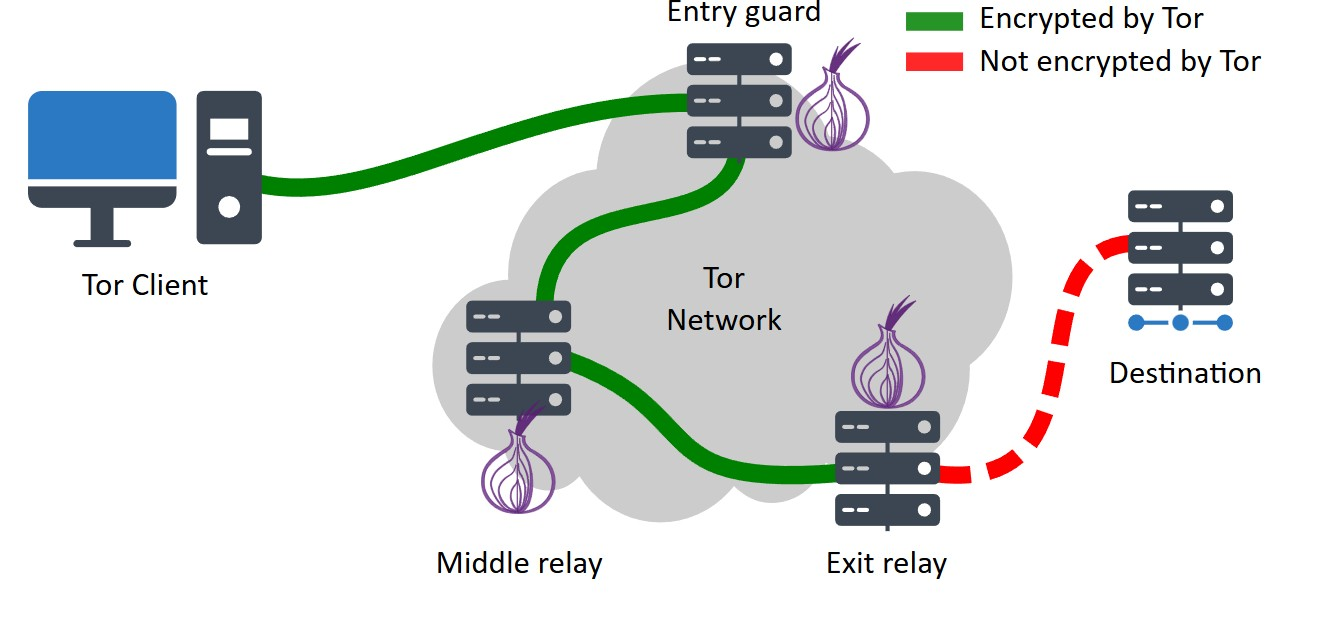
\includegraphics[width=480pt]{Griff/TCD SCSS CAPSTONE/Literature Review/How tor works.jpg}}

\centerline{\textit{Figure 1.2, How the Tor Network Works}}

Tor is a great tool to combat censorship. Tor's distributed architecture of nodes makes it resilient against localized censorship efforts. In countries where the Tor network is blocked, users are able to use "Bridges", which are Tor nodes that are not listed publicly. Using a bridge address allows for the user to connect to the network covertly \cite{torprojectBRIDGESProject}. Users can also avail of "Pluggable transports", which transforms Tor traffic to look like regular network traffic. This method can help circumvent censorship in regions that use \textit{Deep Packet Inspection} (DPI) and other forms of advanced internet censorship \cite{torprojectCIRCUMVENTIONProject}.

\subsection{VPNs}

Virtual Private Networks (VPNs) broadly speaking provide an end-to-end encrypted connection between your device and a VPN server. This method hides your IP address and grants the user anonymity while browsing over the network. This allows users to bypass censorship by connecting to servers outside of their location while masking their IP address \cite{TomsGuideVPN}.

\subsection{Proxies}

A proxy server is similar to a VPN as it fetches content on behalf of a user. When using a proxy, a user can request blocked content via a server in a non-censored region. From the perspective of the censor, the user is only connecting to the proxy server (which is ideally not blocked) and not the actual blocked content. For example, when \textit{The Pirate Bay} was blocked by EIRCOM in Ireland in 2009 by court order, the website was still accessible via proxy servers \cite{PirateBayBlocked2009}.

\subsection{Psiphon VPN}

Psiphon is an open-source internet censorship circumvention tools developed at the Citizen Lab at the University of Toronto. Psiphon uses a combination of VPN, SSH, and Proxy techniques to gives users unfiltered access to the internet. The tool works by attempting to establish a secure tunnel though its distributed network of servers. Once a connection is established, internet traffic is routed through the Psiphon infrastructure. This method circumvents network-level censorship mechanisms such as IP Blocking, DNS Interference, and some forms of Deep Packet Inspection. 

The Open Observatory of Network Interference (OONI) Probe has a built in function to test if the Psiphon tool is blocked within a given network.